\documentclass[journal]{IEEEtran}
\usepackage{amsmath,amssymb}
\usepackage{graphicx}
\usepackage{cite}
\usepackage{booktabs}
\usepackage{multirow}
\usepackage{array}
\usepackage{url}
\usepackage{balance}
\usepackage{siunitx}
\usepackage{xcolor}
\usepackage{hyperref}
\hypersetup{hidelinks}
\graphicspath{{figures/}}

% Match the base journal's hierarchy while retaining the IEEE two-column layout.
\makeatletter
\renewcommand{\thesection}{\arabic{section}}
\renewcommand{\thesubsection}{\Alph{subsection}}
\renewcommand{\thesubsubsection}{\arabic{subsubsection}}
\def\@seccntformat#1{\csname the#1\endcsname.\hspace{0.55em}}
\def\section{\@startsection{section}{1}{\z@}%
  {-1.55ex plus -0.4ex minus -0.2ex}%
  {0.85ex plus 0.15ex}%
  {\normalfont\bfseries\raggedright\fontsize{11}{13}\selectfont\MakeUppercase}}
\def\subsection{\@startsection{subsection}{2}{\z@}%
  {-1.25ex plus -0.3ex minus -0.2ex}%
  {0.55ex plus 0.1ex}%
  {\normalfont\bfseries\fontsize{10}{12}\selectfont}}
\def\subsubsection{\@startsection{subsubsection}{3}{\z@}%
  {-1.0ex plus -0.2ex minus -0.1ex}%
  {0.35ex plus 0.1ex}%
  {\normalfont\bfseries\itshape\fontsize{9.5}{11}\selectfont}}
\makeatother

\begin{document}

\title{A Graph Reinforcement Learning Framework for Routing in a Hybrid Fiber and Free-Space QKD Network}

\author{Author~Names~Withheld~for~Draft% replace before submission
\thanks{This manuscript is a working draft based on the QKD routing simulator maintained by the authors. Author affiliations, funding, and correspondence details are to be completed.}}

\maketitle

\begin{abstract}
Hybrid quantum key distribution (QKD) networks require routing decisions to account for changing link quality and trusted-node constraints. This work presents a simulation framework combining a hybrid fiber and free-space optical (FSO) topology, scenario-based channel models, constrained next-hop selection, and a graph neural network policy trained with proximal policy optimization. The current implementation represents secret-key generation with a normalized rate proxy and evaluates single source-destination route episodes. In one archived Mumbai-to-Kolkata monsoon-night condition, the GNN policy completed 10 of 10 episodes, with a mean of 25.6 hops. This is a preliminary simulator observation and does not establish superiority over conventional routing. A controlled link-choice diagnostic found that the trained policy did not select the higher-rate candidate link, motivating policy and feature ablations. We describe the simulator, its security-model boundaries, and its evaluation protocol, and identify the demand-level and absolute-rate components required for a full network-routing comparison.
\end{abstract}

\begin{IEEEkeywords}
Quantum key distribution, trusted-node networks, routing, graph neural networks, attention, proximal policy optimization, free-space optical communication.
\end{IEEEkeywords}

\section{Introduction}
Quantum key distribution (QKD) supplies shared secret key material using quantum communication and authenticated classical post-processing. Interest in QKD has grown alongside the prospect of quantum algorithms that threaten some public-key systems \cite{shor1997}. In a trusted-node network, intermediate nodes relay key material between distant endpoints. The resulting network routing problem must account for link quality and the availability of stored key material, in addition to conventional path length and hop count \cite{scarani2009,mehic2020,johann2024,munro2015,ituY3800}. The usable rate is constrained by the weakest link on a relayed path, while changing channel conditions can make a route that was feasible at one time infeasible later.

Prior work has compared routing policies for meshed trusted-node networks under traffic and key-store models, including methods with different levels of information available to the controller \cite{johann2024}. Separately, finite-key analysis for simplified trusted-node (STN) chains establishes that security and computational cost depend on protocol details and block size \cite{krawec2024}. These two lines of work motivate a routing study that models link uncertainty and preserves a clear boundary between network-level route selection and cryptographic security proofs.

This paper describes an extensible simulator and a graph-based routing agent for a hybrid fiber and free-space optical (FSO) QKD network. We represent routing as a partially observed sequential decision problem. An agent observes current route state and link features, selects a feasible adjacent node, and receives reward shaped by progress, link utility, security constraints, and route costs. A graph neural network (GNN) encodes node and edge context, while proximal policy optimization (PPO) trains the policy from simulator interaction \cite{schulman2017,kipf2017,velickovic2018}. The implementation includes a hard action mask for invalid QBER/SKR links and supports an optional attention based candidate-scoring component.

The current contribution is methodological and software oriented. It includes: 1) a road-corridor proxy topology for seven Indian city hubs, with candidate FSO bypasses; 2) a layered fiber and FSO link simulator with time-varying, temporally correlated FSO turbulence; 3) a configurable asymptotic secret-key-rate proxy and an opt-in vacuum-plus-weak-decoy finite-key engineering estimator; 4) a masked graph-policy training and evaluation workflow; and 5) an evidence ledger and validation protocol that separate derived simulation outputs from measurements. The present results are limited to archived simulator experiments. They do not establish deployed-network performance, composable finite-key security, or field availability.

The paper is organized as follows. Section II formulates the routing setting and summarizes the QKD model. Section III describes the simulator and evaluation setup. Section IV presents the learned routing policy and comparator formulations. Section V reports preliminary route-level results. Section VI discusses the limits of the current evidence and the requirements for a network-level study. Section VII concludes the paper.

\section{Problem Formulation and QKD Model}
\subsection{Basic Principles of QKD}
QKD protocols combine a quantum channel with authenticated classical communication. BB84 uses nonorthogonal signal states to allow the communicating parties to estimate disturbance and distill key material \cite{bennett1984}. Practical transmitters commonly use weak coherent pulses rather than ideal single-photon sources. Decoy-state methods use pulses with different intensities to estimate single-photon contributions and counter photon-number-splitting attacks \cite{hwang2003,lo2005}.

Finite-key operation must include statistical fluctuations, error-correction leakage, and security parameters. Asymptotic rate formulas are useful for link-level screening, but they do not by themselves certify a finite block. Entropic uncertainty and composable security analyses provide established foundations for finite-size bounds \cite{gllp2004,tomamichel2012,lim2014}. For STN chains, the parties and parity announcements couple information across links. A finite-key bound for such a chain is therefore protocol-specific and cannot be replaced by summing independent per-link asymptotic rates \cite{krawec2024}.

\subsection{Generation and Relaying of Secret Keys}
In a conventional trusted-node chain, neighboring QKD modules establish link keys. The network forwards end-to-end key material through trusted relays, commonly using one-time-pad operations. For a path with link key rates $R_i$, the instantaneous end-to-end service rate is limited by the slowest required resource, and practical delivery also depends on stored key inventory and demand. Key pools therefore couple routing decisions over time \cite{ituY3803,johann2024}.

The simulator's default link utility is a normalized rate proxy, not a throughput in bits per second. A fiber channel is attenuated as a function of distance, and a detector model contributes efficiency and dark counts. The code computes a QBER proxy and a rate proxy from these quantities. The optional finite-key BB84 mode adds decoy-state and uncertainty terms, but has not been independently verified as a composable proof against measured detection counts. Fig. 1 illustrates the configured distance-dependent proxy under selected channel scenarios.

\begin{figure}[t]
\centering
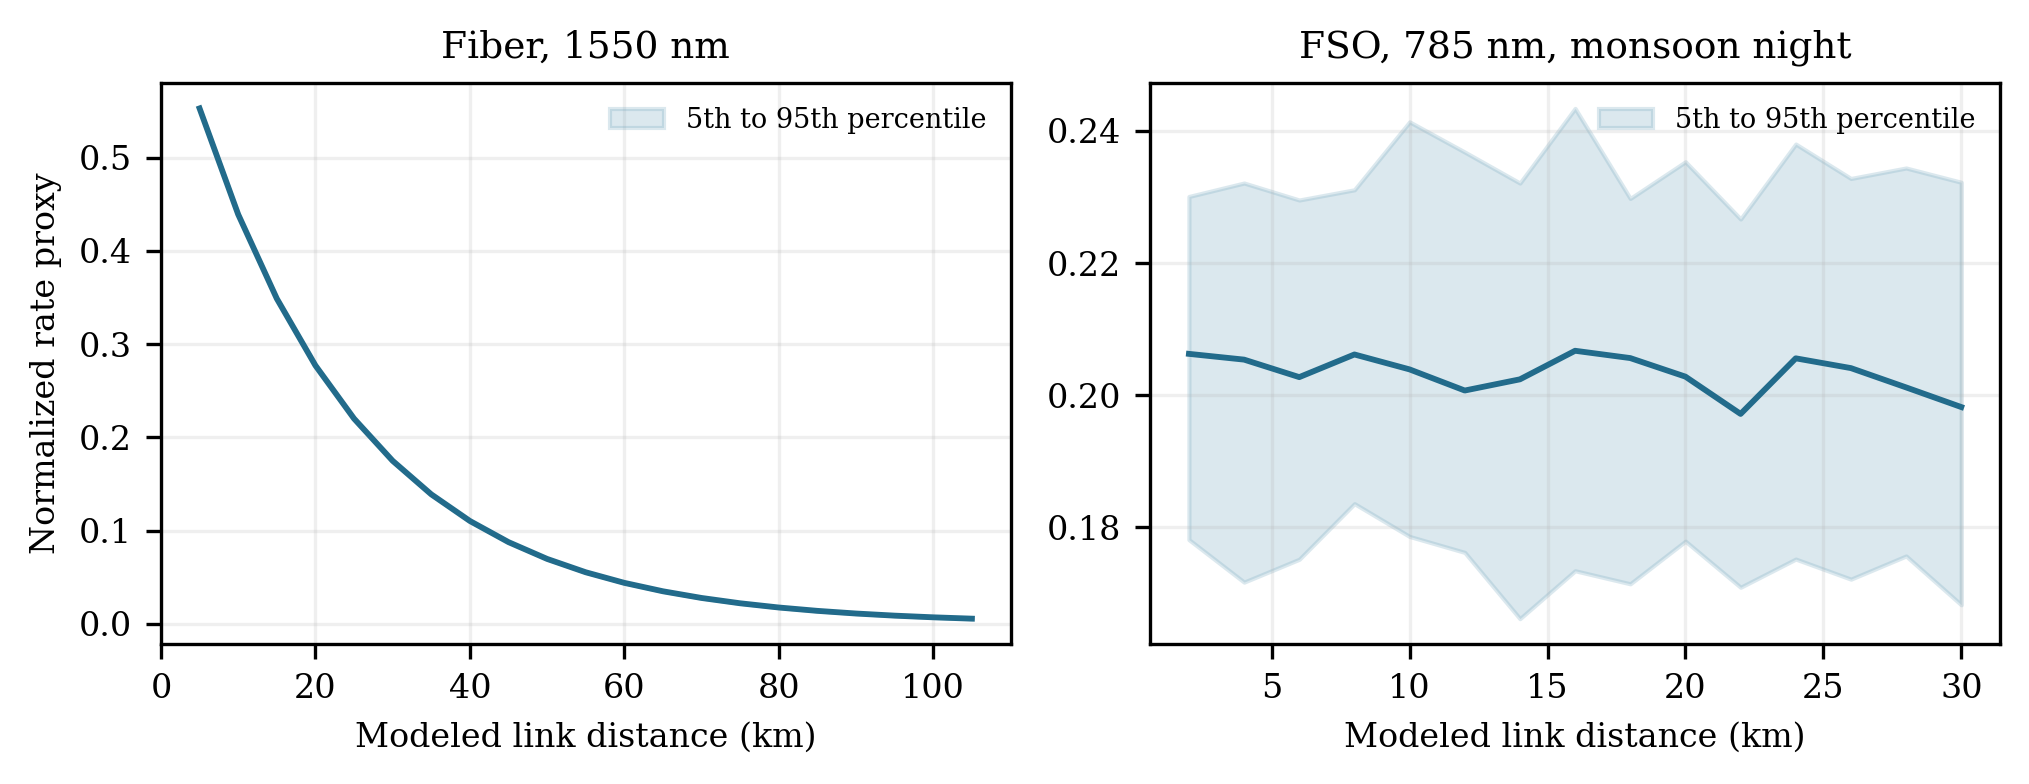
\includegraphics[width=\columnwidth]{rate_distance.png}
\caption{Modeled normalized rate proxy versus link distance for the configured fiber and FSO scenarios. Shading shows sampled scenario variation, not measured uncertainty or validation against a published curve.}
\label{fig:ratedistance}
\end{figure}

In a conventional trusted-node (TN) chain, each neighboring pair performs QKD and the intermediate TNs relay link keys. Each TN is trusted with the key material it handles. In a simplified trusted-node (STN) chain, intermediate devices can perform state preparation or measurement and announce parities of raw link data, while error correction and privacy amplification are performed by the end users. The security analysis therefore treats the whole chain and its correlated public announcements, rather than assigning an independent single-link proof to every hop. Krawec \emph{et al.} derive a finite-key bound for this STN setting and analyze its cost trade-off against conventional TN chains \cite{krawec2024}. In this project, that proof is background motivation only: the implemented estimator is not their chain proof, and the simulated relay types do not establish a composable security guarantee.

\begin{figure}[t]
\centering
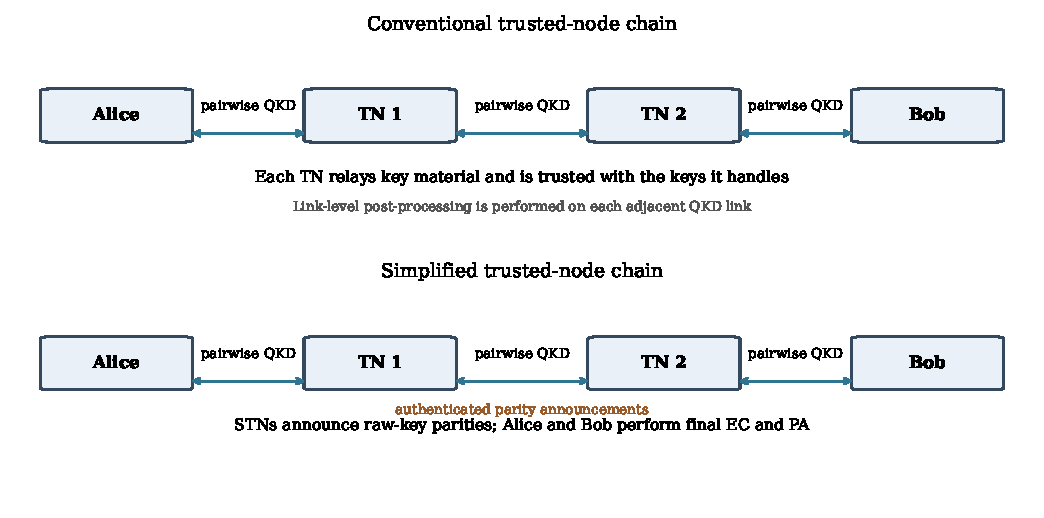
\includegraphics[width=\columnwidth]{tn_stn_relay.pdf}
\caption{Conceptual key-relay roles in conventional TN and STN chains. The STN security proof is cited background and is not implemented by the simulator.}
\label{fig:tnstn}
\end{figure}

\subsection{Application of QKD to Meshed Networks}
Long fiber spans motivate intermediate trusted nodes. FSO links can provide candidate bypasses where a direct fiber span is unavailable or degraded. Their channel quality depends on atmospheric attenuation, turbulence, pointing, and availability. Terrestrial FSO design methods identify these as separate budget terms and require local environmental information for credible planning \cite{ituP1814,krzic2023}. The simulator models time-of-day and seasonal scenario variables, but its current FSO distributions are assumptions rather than fits to site-specific Indian weather traces.

\subsection{State of the Art in QKD Routing}
Classical shortest-path methods provide reproducible baselines but typically optimize a fixed edge cost \cite{dijkstra1959}. QKD network studies also consider key-store utilization, request blocking, load balancing, and management overhead \cite{mehic2020,johann2024}. Recent learning-based work has applied PPO to entanglement routing in quantum communication networks and state-dependent routing to networks combining trusted nodes and repeaters \cite{roik2024routing,amer2023dynamic}. These settings differ from trusted-node key-pool routing with hybrid fiber and FSO links, so their results do not validate the present simulator. In dynamic settings, sequential decision methods can account for state-dependent link availability, with dynamic programming providing a classical foundation for sequential optimization \cite{bellman1957}. PPO is a clipped policy-gradient method that supports repeated minibatch updates from sampled rollouts \cite{schulman2017}; generalized advantage estimation reduces variance in return estimates \cite{schulman2016gae}. The partially observed formulation follows standard POMDP and reinforcement-learning foundations \cite{kaelbling1998,sutton2018}.

GNNs represent relationships among nodes and edges through message passing. Graph convolution provides a compact aggregation rule \cite{kipf2017}; inductive neighborhood aggregation and general message-passing formulations provide related design patterns \cite{hamilton2017,gilmer2017}. Attention mechanisms allow learned weighting of neighborhood information \cite{vaswani2017,velickovic2018}. These properties are relevant when one policy must operate on a network graph and select among adjacent actions. They do not guarantee that the agent learns a physically appropriate link preference, which must be evaluated with controlled tests.

\section{Simulator Architecture and Experimental Setup}
\subsection{Architecture}
The simulator has four logical components: topology and link profiles, a time-stepped environment, a routing policy, and an evaluation layer. The topology represents QKD-capable sites and candidate communication links. The environment samples channel conditions, enforces link security and reachability constraints, tracks route history and key-pool state, and returns an observation and reward. The policy selects a next-hop action. Evaluation replays fixed seeds and compares learned policies with conventional baselines. The present software does not implement a production key-management plane or a QKD device control interface.

\begin{figure}[t]
\centering
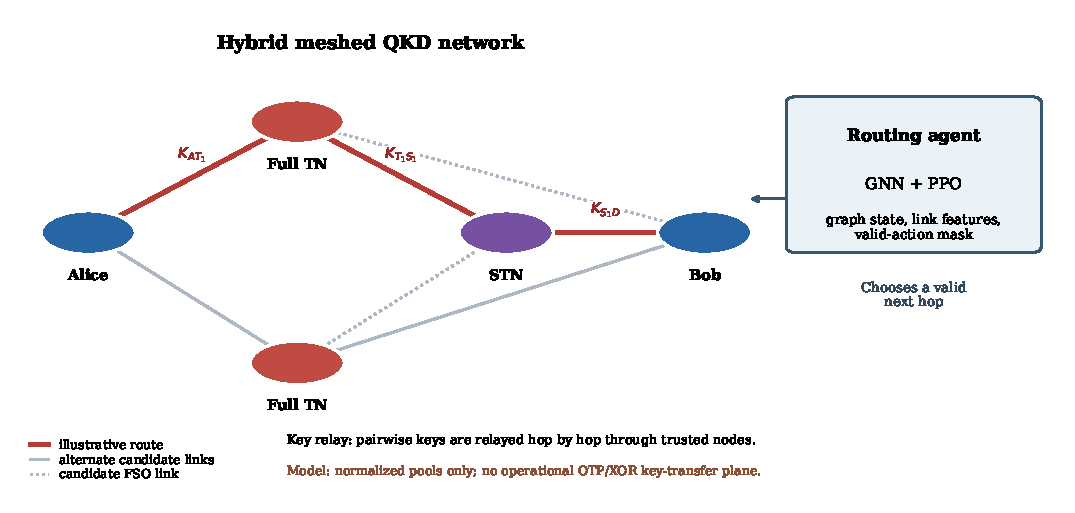
\includegraphics[width=\columnwidth]{meshed_key_relay_architecture.pdf}
\caption{Hybrid meshed QKD routing and key-relay schematic. Red links show an illustrative multihop route with per-link key labels; gray links show alternatives. The controller represents the centralized graph observation used in simulation. Key transfer and the OTP/XOR relay plane remain conceptual abstractions.}
\label{fig:architecture}
\end{figure}

\subsection{Security Requirements on the Network Controller}
The reference architecture assumes a controller with topology and link-health information. This manuscript distinguishes a local policy that acts on its current observation from a centralized oracle that can inspect a fixed simulated network state. In a deployed QKD network, telemetry on key-pool levels and link health would need authenticated and integrity-protected control channels. The current simulator does not implement a network controller protocol, attacks on telemetry, or a control-message counter. Thus, management overhead and telemetry security are architectural requirements, not measured outcomes here.

\subsection{Simulation Setup}
\subsubsection{Topology and Corridor Data}
The current topology uses seven city hubs: Delhi, Jaipur, Mumbai, Bangalore, Hyderabad, Kolkata, and Chennai. OpenStreetMap driving routes provide candidate fiber-corridor geometry. These routes are planning proxies, not verified operator fiber routes, surveyed alignments, or guaranteed rights-of-way. The graph contains 2,370 modeled nodes and 2,653 links, including 273 fiber links and 2,380 candidate FSO links. FSO line of sight, terrain clearance, and access to physical infrastructure are not verified. Topology geometry is archived with the research data. OpenStreetMap data use is governed by its applicable attribution and database terms \cite{osm2008}.

\begin{figure}[t]
\centering
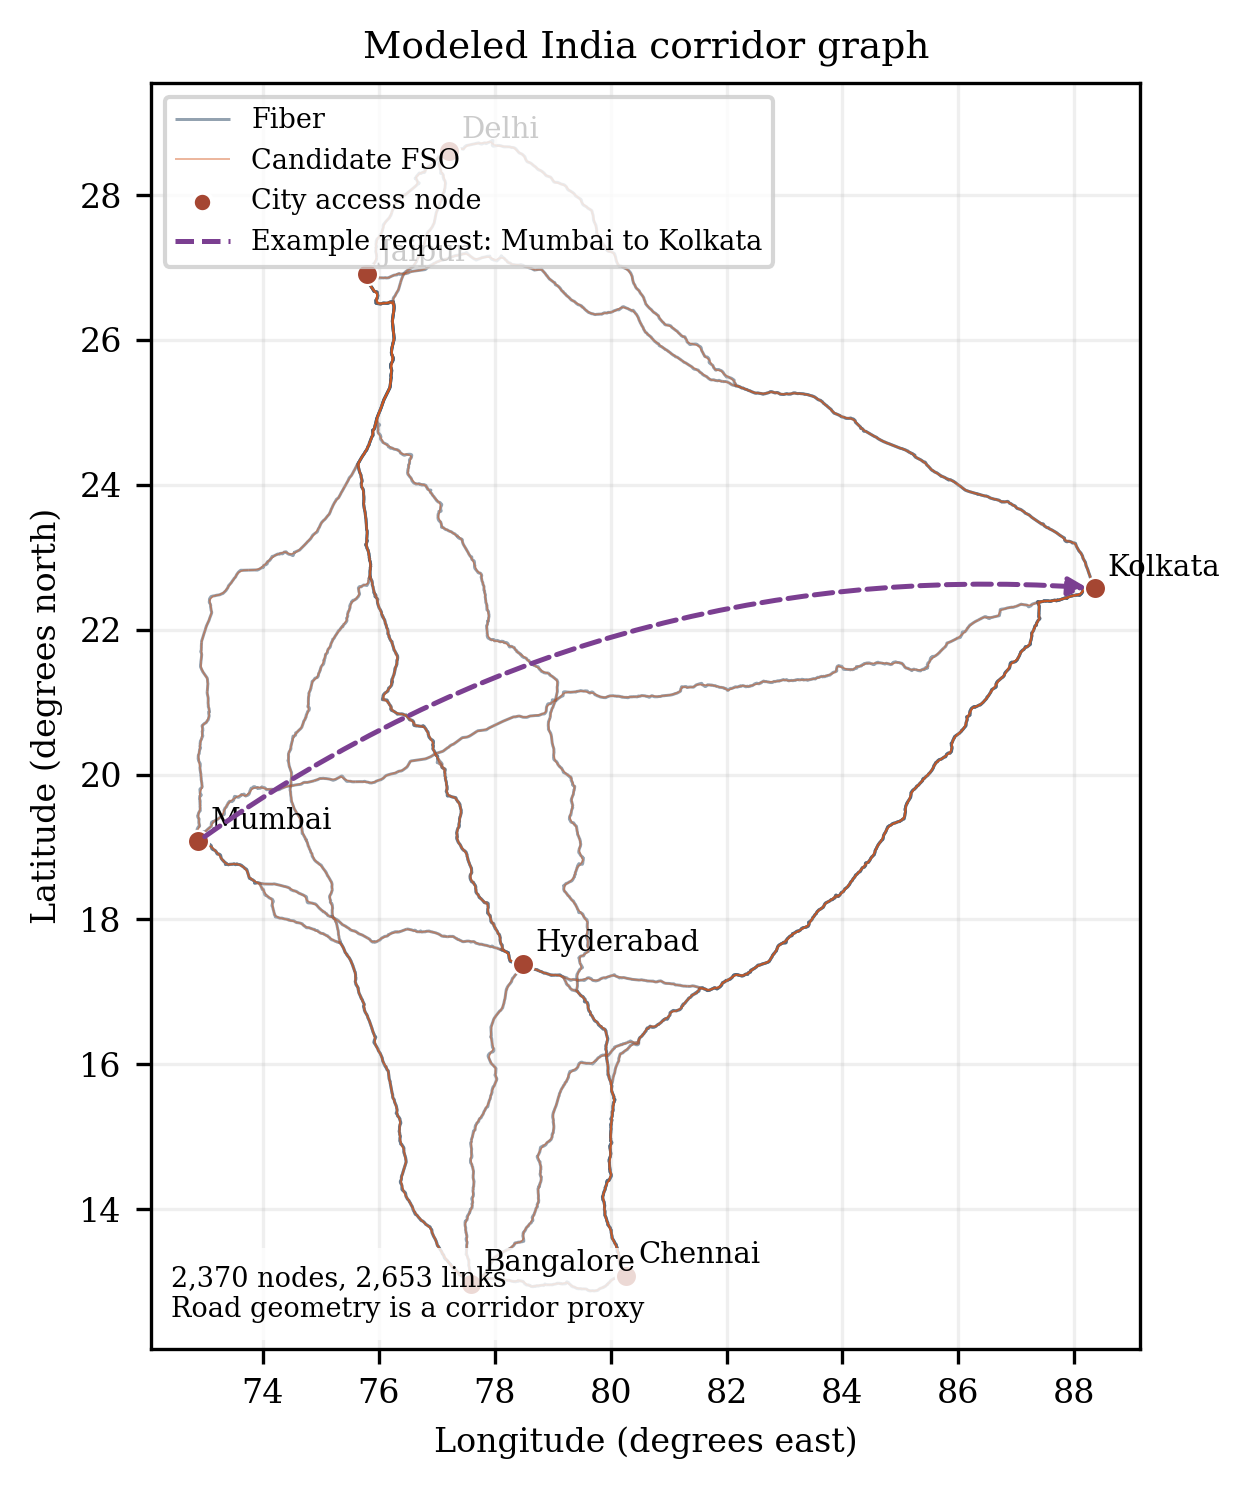
\includegraphics[width=\columnwidth]{corridor_map.png}
\caption{Modeled corridor graph with fiber links and candidate FSO links. The dashed Mumbai-to-Kolkata line marks an example request, not a physical link. Road geometry is a corridor proxy; FSO line of sight is assumed.}
\label{fig:map}
\end{figure}

\subsubsection{Link and Noise Models}
Fiber loss is represented using wavelength-dependent attenuation and excess loss. Detector efficiency, dark-count bounds, and a visibility assumption contribute to detection and QBER proxies. The selected fiber device profile is based on published/vendor-reported ID Quantique ID281 values at 1550 nm. The FSO channel is a separate assumed 785-nm scenario with its own efficiency and dark-count settings. These are not a single matched commercial optical terminal profile.

\begin{table}[t]
\caption{Representative link-model parameters and evidence class}
\label{tab:physical}
\centering
\scriptsize
\begin{tabular}{p{0.27\columnwidth}p{0.31\columnwidth}p{0.32\columnwidth}}
\toprule
Quantity & Configured value & Evidence class\\
\midrule
Fiber wavelength & 1550 nm & device profile\\
Fiber attenuation & 0.20 dB/km & inherited target\\
Fiber detector efficiency & 0.93 & measured device value\\
Fiber dark-count bound & $<70$ s$^{-1}$ & measured upper bound\\
FSO wavelength & 785 nm & scenario assumption\\
FSO detector efficiency & 0.60 & scenario assumption\\
FSO dark counts & 100 s$^{-1}$ & scenario assumption\\
FSO temporal correlation & 0.85 & uncalibrated assumption\\
\bottomrule
\end{tabular}
\end{table}

FSO turbulence is represented with a correlated latent log-$C_n^2$ process. The environment samples availability and channel conditions by time step; FSO corridor outages are held fixed for the episode to avoid a bypass disappearing between its relay segments. These choices create repeatable stress scenarios. They are not observations of weather on the modeled routes. A detailed parameter ledger and provenance categories are supplied in \texttt{PHYSICS\_EVIDENCE.md}.

The implemented FSO model uses a correlated log-normal turbulence process with atmospheric, diffraction, pointing, and background terms. It does not implement a Gamma-Gamma irradiance model or a generalized amplitude-damping channel. Detector and channel noise enter through the project's QBER and rate calculations. Fig. 5 summarizes this implemented coupling; the optional finite-key estimator remains a simplified engineering model.

\begin{figure}[t]
\centering
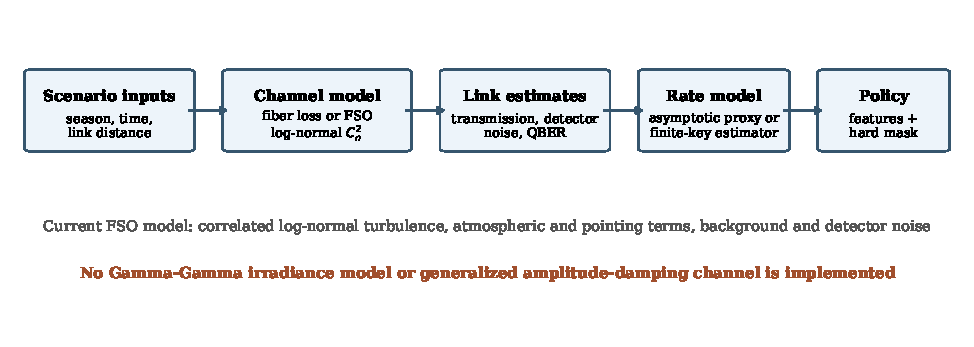
\includegraphics[width=\columnwidth]{physics_to_policy.pdf}
\caption{Implemented channel-to-routing coupling. The figure distinguishes the current log-normal scenario model from other turbulence and quantum-channel models that are not implemented.}
\label{fig:physcoupling}
\end{figure}

The default rate mode is an asymptotic, normalized proxy of the form
\begin{equation}
 r_{\mathrm{proxy}} = p_{\mathrm{det}}\left[1-2h_2(Q)\right],
 \label{eq:proxy}
\end{equation}
where $p_{\mathrm{det}}$ is modeled detection probability, $Q$ is modeled QBER, and $h_2$ is binary entropy. The expression is used only as a simulator utility. It is not a composable key rate, does not include all protocol terms, and is not reported in bits per second. An opt-in decoy-state mode estimates finite-key contributions and uncertainty, but that mode is also not a formal security certificate.


\subsubsection{Environment and Protected Conditions}
At each time step the observation contains the current node, destination-relative distance, node type, normalized degree, candidate link features, and route history features. Absolute coordinates and node identifiers are excluded from the configured relative feature mode. Candidate actions are limited to adjacent nodes. Links that violate the hard QBER threshold or have invalid rate are masked before action sampling. The threshold is configured at $Q_{\max}=0.11$.

The reward includes destination progress, distance-aware link utility, a step cost, revisit and link-switch penalties, a backtracking penalty, and explicit security and key-pool depletion penalties. The link utility is prorated by modeled link distance so subdividing a span does not multiply its total rate reward. The experimental protocol records these as protected or adjustable values and stores resolved configurations with each run.

The observation contains five node features and nine features for each candidate edge. For the archived run, node inputs use destination-relative distance and normalized degree, while edge inputs use the simulator quantities listed in Table~\ref{tab:features}. The defence reward profile uses weights $w_{\mathrm{progress}}=0.2$, $w_{\mathrm{margin}}=0.8$, $w_{\mathrm{SKR}}=1.2$, $w_{\mathrm{pool}}=0.4$, $w_{\mathrm{latency}}=0.4$, $w_{\mathrm{energy}}=0.4$, $w_{\mathrm{congestion}}=0.5$, and destination bonus $4.0$. Additional configured penalties are $-0.05$ per step, $-0.6$ for a revisit, $-0.2$ for switching link type, $-0.5$ for backtracking, $-30$ for a security breach, and $-60$ for pool depletion.

\begin{table}[t]
\caption{Observation features for each current node and candidate edge}
\label{tab:features}
\centering
\scriptsize
\begin{tabular}{p{0.2\columnwidth}p{0.72\columnwidth}}
\toprule
Feature group & Components\\
\midrule
Node (5) & City indicator; full-TN indicator; STN indicator; destination-relative distance; normalized degree.\\
Edge (9) & QBER; normalized secret-key-rate proxy; FSO indicator; normalized distance; projected chain error; normalized key-pool state; link-type switch; visited-node flag; destination-distance progress.\\
Action mask & Edge is adjacent, passes the edge QBER threshold, has positive modeled rate, and remains below the projected chain-error threshold.\\
\bottomrule
\end{tabular}
\end{table}

\subsubsection{Training and Evaluation Setup}
The GNN policy uses three message-passing layers, a shared actor-critic trunk, and a masked action head. The implementation uses a monotone log-rate prior and an explicit distance-progress prior. Behavior cloning can initialize the policy from shortest-path demonstrations before PPO fine-tuning. PPO uses clipped policy updates, generalized advantage estimation, reward normalization, gradient clipping, and checkpointed normalization state. The optional attention model is implemented in \texttt{qkd\_attention.py}; the GNN-PPO runs summarized below use the graph policy configuration specified in their saved YAML files.

\begin{table}[t]
\caption{Archived GNN-PPO evaluation scenario}
\label{tab:scenario}
\centering
\scriptsize
\begin{tabular}{p{0.43\columnwidth}p{0.46\columnwidth}}
\toprule
Setting & Value\\
\midrule
Source and destination & Mumbai to Kolkata\\
Season and start time & Monsoon, 22:00 $\pm$ 1 h\\
Training budget & 200 PPO epochs, resumed checkpoint\\
Hidden dimension & 64\\
Evaluation seeds & 10\\
QBER hard threshold & 0.11\\
Fiber outage probability & 0.01\\
\bottomrule
\end{tabular}
\end{table}

Baselines include random feasible action selection, shortest distance with Dijkstra, breadth-first hop count, and maximum instantaneous rate. Baseline outcomes are sensitive to whether they observe current rates, how they break ties, and how repeated states are handled. Each comparison must therefore use a common environment, endpoint pair, seed set, termination rule, and action feasibility mask. The packaged experiment protocol identifies the controlled conditions and required diagnostics.

\begin{figure}[t]
\centering
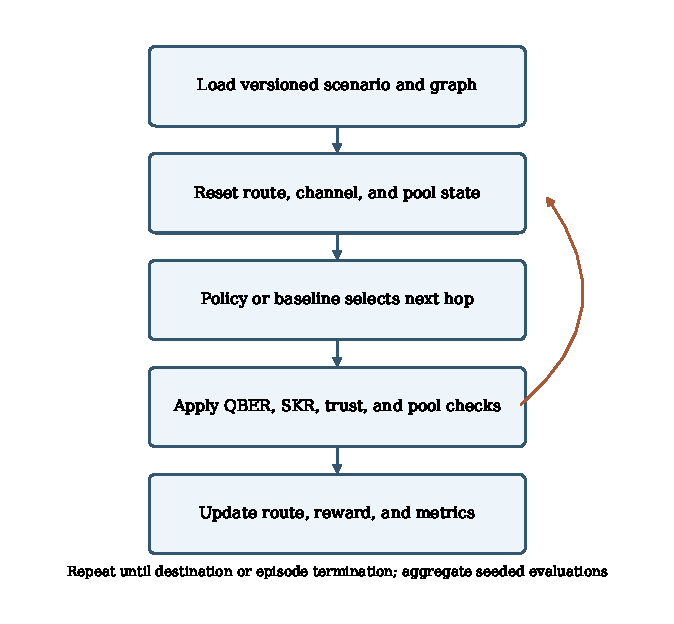
\includegraphics[width=0.82\columnwidth]{simulation_flow.pdf}
\caption{Simulation and evaluation flow used by the routing environment. The diagram describes the implemented single-route experiment loop.}
\label{fig:simflow}
\end{figure}

\section{Routing Policy and Learning Objective}
\subsection{Hop-Count Comparator}
The hop-count comparator uses breadth-first search over the modeled topology. Prior trusted-node routing studies evaluate multiple loopless $k$-shortest paths and check key-store feasibility on each candidate. The present baseline selects a next hop and does not implement that $k$-candidate buffer-feasibility procedure. It is a topology-routing comparator rather than a demand-level key-pool algorithm.

\subsection{Perfect-Information Comparator}
An oracle comparator can use future demand or channel-state information unavailable to an online policy. The present simulator has neither a demand matrix nor a future-state evaluation interface, so no perfect-information result is reported.

\subsection{Graph and Sequence Policy Encoders}
The repository provides both an \texttt{LSTMActorCritic} and a GNN-PPO policy. The LSTM is a graph-blind encoder over an ordered node-feature array, not a recurrent demand-history predictor. The GNN-PPO policy operates on the current graph and link observation. The reported experiment uses GNN-PPO; no matched LSTM comparison is included.

\subsubsection{Policy Formulation and PPO Training}
Let the network be a graph $G=(V,E)$, with source $s$, destination $d$, and time-varying state $x_t$. The agent observes $o_t$ and selects an adjacent node action $a_t$ from the feasible set $\mathcal{A}(o_t)$. Transition dynamics sample channel conditions and update route and key-pool state. Because future turbulence and outages are not exposed to the policy, the routing task is partially observed.

The objective is to find a policy $\pi_\theta(a_t\mid o_t)$ that maximizes expected discounted return
\begin{equation}
 J(\theta)=\mathbb{E}_{\pi_\theta}\left[\sum_{t=0}^{T}\gamma^t r_t\right],
 \label{eq:objective}
\end{equation}
subject to hard feasibility constraints on link adjacency, QBER, and modeled key availability. The reward is a training signal; reported evaluation metrics include route success, successful-route hop count, revisits, QBER/rate validity, and seed variation. A reward value alone is not interpreted as network service quality.

\subsubsection{Graph Policy and Action Mask}
For each node $v$, the message-passing stack computes an embedding $h_v$ from the node state and valid neighboring features. The actor produces logits $z_{v,u}$ for adjacent candidate actions. Invalid candidates are assigned negative infinity before softmax:
\begin{equation}
 \pi_\theta(u\mid o_t)=\operatorname{softmax}_{u\in\mathcal{A}(o_t)}(z_{v_t,u}).
\end{equation}
Invalid links contribute no message in either direction. This separates the safety constraint from the learned preference: training cannot select a currently invalid edge, while model quality determines which of the remaining edges is chosen.

In the optional attention variant, candidate embeddings are combined using learned compatibility scores, following neighborhood attention formulations \cite{velickovic2018}. Attention is treated as an architectural choice. Its value must be established by an ablation with the same training budget and seed distribution. The current results do not isolate a causal benefit from attention.

\begin{figure}[t]
\centering
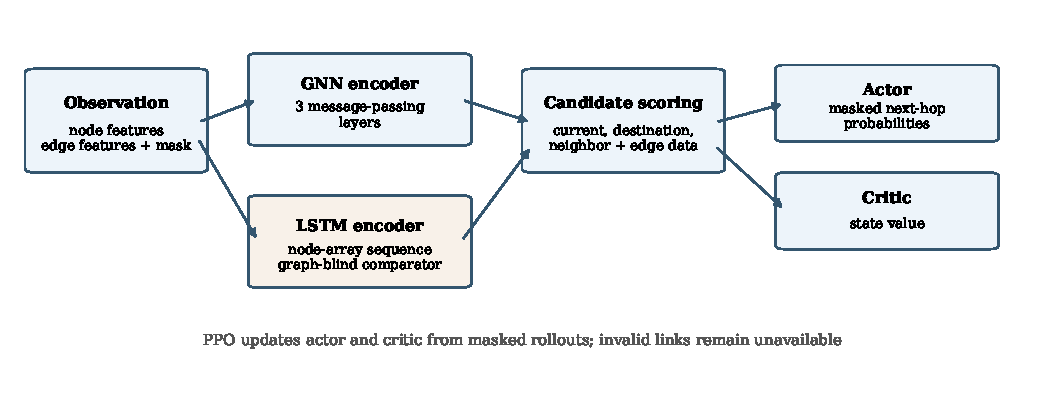
\includegraphics[width=\columnwidth]{gnn_ppo.pdf}
\caption{GNN-PPO policy architecture and the available graph-blind LSTM encoder comparator. The LSTM input is an ordered node-feature array, not a time-series demand forecast.}
\label{fig:policy}
\end{figure}

\subsubsection{PPO Training}
The policy is updated by maximizing the clipped surrogate objective
\begin{equation}
 L^{\mathrm{clip}}(\theta)=\mathbb{E}_t\left[\min\left(\rho_t(\theta)\hat A_t,
 \operatorname{clip}(\rho_t(\theta),1-\epsilon,1+\epsilon)\hat A_t\right)\right],
\end{equation}
where $\rho_t(\theta)$ is the new-to-old action probability ratio and $\hat A_t$ is the estimated advantage. PPO is combined with a value loss and entropy regularization. Hyperparameters are resolved from a versioned YAML file and included with the experiment artifact. The specific settings for the preliminary run are in the supplementary package.

\subsection{Centralized Comparator Formulations}
A centralized link-weight comparator can assign edge costs from link state and key-pool information, while an integer linear program can optimize simultaneous demands subject to link capacities. The current single-route simulator does not provide the demand matrix or calibrated key generation and consumption units needed to evaluate either method on a shared objective. These comparator families are outside the measured experiment reported here.

\subsubsection{Link-Weight Optimization}
A published trusted-node routing heuristic sets an edge weight from key-store emptiness $E_e$ as $W_e=\exp(aE_e)$, with tuning parameter $a$ \cite{johann2024}. A rate-aware extension could include an inverse-rate term, but that would define a different method. The present simulator has no demand stream or multi-demand key-store dynamics, so neither heuristic is included in the measured evaluation.

\subsubsection{Integer Linear Programming}
For completeness, a demand-level oracle can be written using binary variable $x_{kp}$, which is one when request $k$ is assigned candidate path $p$, request demand $b_k$, and edge key availability $C_e$. The standard capacity-constrained formulation is
\begin{align}
\max_{x_{kp}}\quad & \sum_{k\in\mathcal{K}}\sum_{p\in\mathcal{P}_k} x_{kp},\\
\mathrm{s.t.}\quad & \sum_{p\in\mathcal{P}_k}x_{kp}\leq 1,\quad k\in\mathcal{K},\\
& \sum_{k\in\mathcal{K}}\sum_{p\in\mathcal{P}_k:e\in p}b_kx_{kp}\leq C_e,\quad e\in\mathcal{E},\\
& x_{kp}\in\{0,1\}.
\end{align}
The current environment processes one route episode and lacks a time-indexed request matrix and calibrated key-store refill process. This ILP is therefore a mathematical comparator definition, not a measured result.

\section{Preliminary Results}
\subsection{Route Completion and Baseline Behavior}
The archived comparison used the road-corridor graph, Mumbai as source, Kolkata as destination, monsoon conditions, a nominal 22:00 start with one-hour jitter, and ten evaluation seeds. The GNN model had 200 PPO epochs and was resumed from the archived 100-epoch checkpoint. An independent NetworkX search of the current topology confirms a 24-edge unweighted shortest path between these hubs. The previously stored 23-edge reference was incorrect. The GNN mean of 25.6 hops comes from that archived run and is not evidence of optimality.

The archived GNN completed all ten recorded episodes. The baseline rows in the old comparison were produced by a selector that did not consistently honor the environment's feasibility mask and are excluded as comparative evidence. The corrected baseline selector now uses the observation's action ordering and valid-action mask. Its episode-level results have not been regenerated because the available Python environments do not include Gymnasium. Thus, only the archived GNN completion count is reported here, and it should be read as a single-condition simulator observation.

\begin{table}[t]
\caption{Archived GNN route outcome for Mumbai-to-Kolkata in the monsoon-night condition. The former baseline outputs are omitted because their selector did not honor the current feasibility mask.}
\label{tab:prelim}
\centering
\footnotesize
\begin{tabular}{@{}p{0.23\columnwidth}p{0.12\columnwidth}p{0.14\columnwidth}p{0.35\columnwidth}@{}}
\toprule
Policy & Success & Mean hops & Result scope\\
\midrule
GNN-PPO, 200 epochs & 10/10 & 25.6 & resumed run\\
\bottomrule
\multicolumn{4}{p{0.88\columnwidth}}{\scriptsize This is a single-condition result from an archived GNN run. It does not establish comparative performance or generalization.}
\end{tabular}
\end{table}

The former baseline results are not included because the selector could choose an action that the environment subsequently replaced through its fallback rule. The revised selector chooses only from currently valid actions. Independent topology checks confirm the 24-edge hop minimum; evaluation on stochastic channel snapshots requires Gymnasium, which is absent from the available runtime.

\section{Discussion and Limitations}
\subsection{Key-Store Utilization}
The environment carries a normalized per-edge pool state and applies modeled depletion and replenishment terms during an episode. It does not represent a 10,000-key initialized buffer or refill from an absolute measured key rate. Since the environment has no multi-demand trace, its pool state cannot support comparable network-wide utilization or load-balancing results.

\subsection{Management Traffic}
The current simulator does not count controller queries, telemetry bytes, or control messages. Management traffic is not measured because neither a central-controller protocol nor local-observation exchange rules are implemented.

\subsubsection{Link Model Characterization}
The stored physics report estimates, at 80 km and 1550 nm, 16.46 dB fiber loss including modeled excess loss, a detection probability of approximately 0.021 per incident photon, QBER proxy of 0.0105, and normalized rate proxy of 0.0175. This calculation uses an idealized one-photon-per-pulse count interpretation for a separate count-rate bound; weak-pulse source statistics are not included in that bound. For a 10-km FSO span during the monsoon 22:00 scenario, the modeled availability was 88\% by configuration and 88.5\% across 1,000 generated samples. Its median normalized rate proxy conditional on sampled available states was 0.2035. These values are generated by assumptions and should not be described as measured link performance.

\begin{figure}[t]
\centering
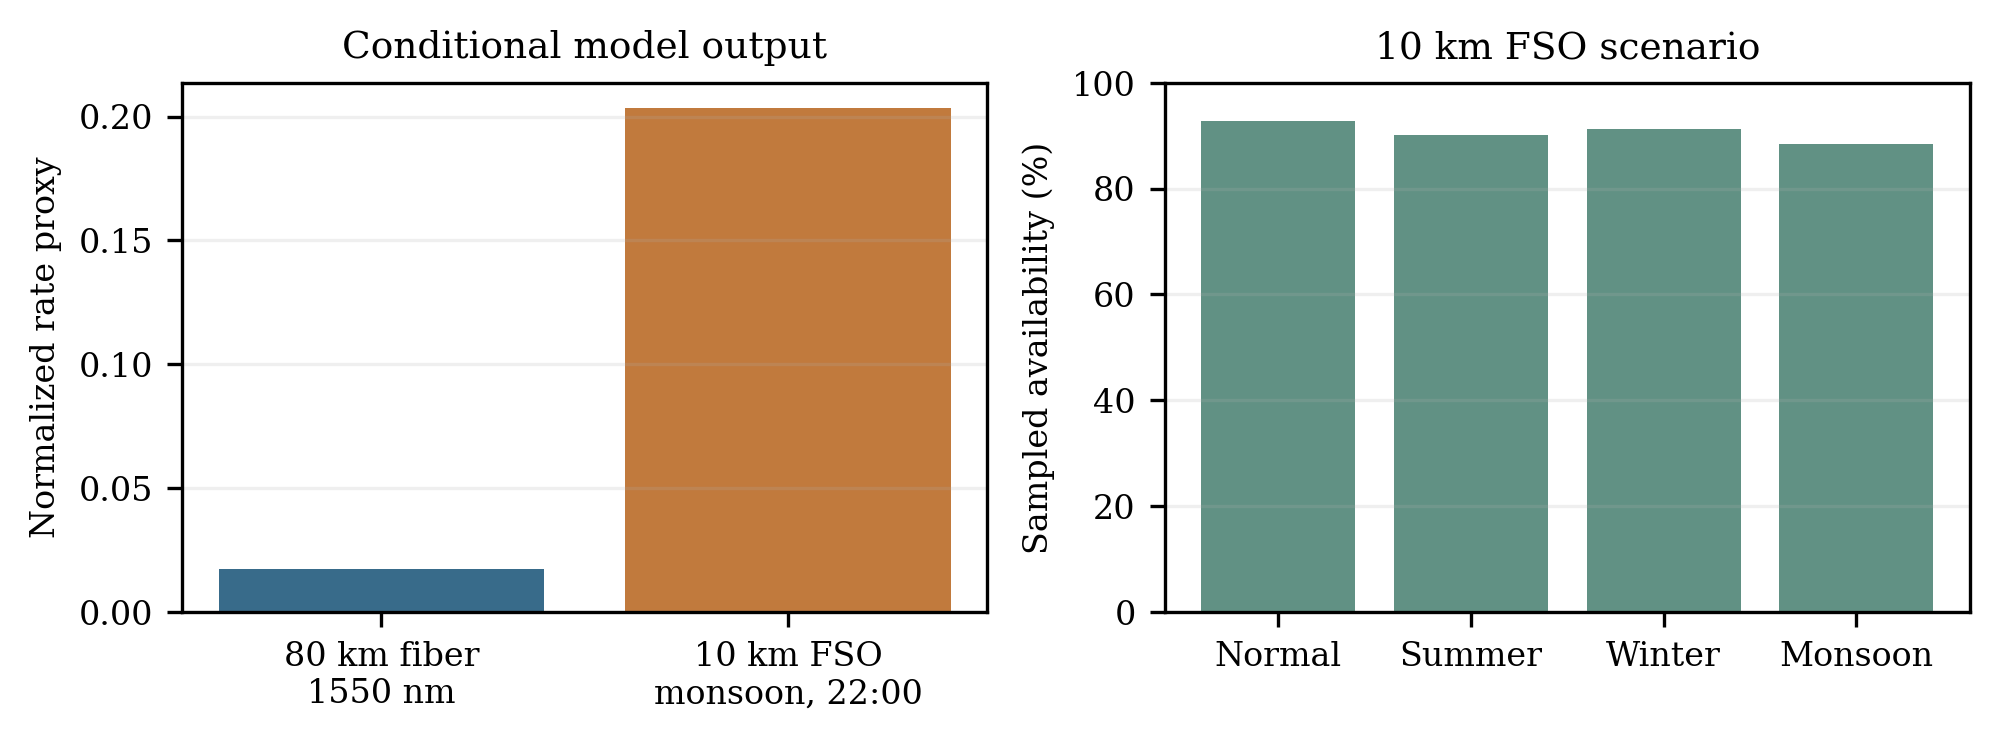
\includegraphics[width=\columnwidth]{link_model_summary.png}
\caption{Selected stored model outputs for fiber and FSO scenarios. Values are derived from the configured simulator, not measured traces.}
\label{fig:link}
\end{figure}

\subsubsection{Controlled Link-Choice Diagnostic}
An archived paired-edge diagnostic compared a modeled 80-km fiber candidate with a clear 10-km FSO candidate while controlling route progress. Across 384 comparisons, the FSO candidate had a higher normalized rate proxy in all sampled pairs. However, the evaluated agent selected the FSO candidate in zero cases, and its assigned action probability remained near one-half. This finding is evidence that the current policy did not demonstrate a useful preference for the higher-proxy candidate under that diagnostic. It also shows that the policy's inclusion of physics-derived features does not establish that those features are used effectively.

\subsection{Scope of the Current Evaluation}
The evaluation covers one trained GNN model and one endpoint pair in one weather condition. It does not estimate variation across independent training runs, endpoint pairs, seasons, or calibrated channel traces. It also does not compare absolute delivered key volume, blocking under traffic, control-plane load, or target-hardware latency. Accordingly, the results characterize a software prototype and not network service performance.

\paragraph{Validation levels.}
Validation is separated into implementation correctness, analytical checks, parameter calibration, synthetic stress testing, and hardware-in-the-loop or field evaluation. Implementation checks cover attenuation, detection, QBER, finite-key bounds, temporal correlation, outage behavior, and path constraints. Analytical validation compares code outputs with limiting cases and independently calculated reference values. Calibration requires traceable device and channel data with uncertainty records. Synthetic testing holds out entire weather traces and applies parameter shifts. Field validation requires timestamped measurements and separate reporting of model error and policy error.

\paragraph{Research use cases.}
The intended research campaigns include: (i) endpoint-pair generalization across the seven city hubs; (ii) seasonal and diurnal FSO robustness, including held-out weather distributions; (iii) demand-weighted routing with key-pool refill and blocking probability; (iv) controlled link choice when candidates trade off distance, rate, and outage risk; and (v) ablations of message passing, attention, behavior cloning, and reward terms. For each study, the unit of replication is a trained model and independent environment seed. Report success and blocking rates with confidence intervals, route length, delivered key bits where defined, QBER threshold violations, revisit rates, calibration error, and inference time. Hyperparameter selection and test seeds must be separated.

\paragraph{Limitations.}
Current road routes are proxies and may not correspond to deployable fiber. FSO visibility and optical geometry are not validated. Weather distributions and effective turbulence scaling are assumptions. The fiber and FSO hardware settings do not represent one fully characterized terminal pair. The default rate expression is a normalized utility, and the finite-key implementation is not independently verified as a composable proof. The simulator supports algorithm development, but this evidence does not establish field performance or certified security.

\section{Conclusion}
This paper has presented a graph-based reinforcement-learning simulator for routing in a modeled hybrid fiber and FSO trusted-node QKD network. The implementation combines constrained next-hop selection, GNN embeddings, PPO training, scenario-based channel variability, and reproducible experiment configurations. In one archived monsoon-night endpoint scenario, the GNN route completed ten of ten episodes. A controlled link-choice diagnostic found that the trained policy did not prefer a higher proxy-rate FSO option. Together, these results define the present prototype's operating scope and expose a link-selection weakness.

Further study requires matched baseline experiments, a demand and absolute key-rate model, independent channel validation, and evaluation across held-out seasons and endpoint pairs. Measured device and channel traces are required before interpreting simulator outputs as network performance. Formal security claims require protocol-specific finite-key analysis and independently checked count data.

\section*{Acknowledgment}
Funding and institutional acknowledgments are to be supplied by the authors.

\section*{Data and Code Availability}
The simulator code, archived configurations, scenario outputs, and generated figures are included with the supplementary research package. The road-corridor geometries derive from OpenStreetMap data and are provided under the Open Database License. Publications using the map should credit ``Map data from OpenStreetMap contributors'' and link to \url{https://www.openstreetmap.org/copyright}. The geometries are routing proxies and do not represent verified fiber infrastructure.

\balance
\bibliographystyle{IEEEtran}
\bibliography{references}

\end{document}
